\chapter{Dialogs}
\label{sec:dialogs}

%%%%%%%%%%%%%%%%%%%%%%%%%%%%%%%%%%%%%%%%%%%%%%%%%%%%%%%%%%%%%%%%%%%%%%%%%%%%%%%%%%%%%%%%%%%%%%%%%%%%%%%%%%%%%%%%%%%%%%%%

\section{Lab Notes}
\label{dlg:labnotes}

The Lab Notes dialog allows you to take notes on your experimental setup. It contains two tabs: ``setup notes"
and "general notes".

The contents of the Setup Notes tab are displayed on the \hyperref[dlg:speedbump]{Speed Bump} dialog when loading a
session file. The General Notes are only displayed within the Lab Notes dialog and are intended purely as a place for
recording interesting observations made during the experiment.

Minimal Markdown syntax (headings and bullets) is currently supported.\footnote{Images and links are supported by the
Markdown renderer library but the integration to properly use them is not yet finished; tables are not supported but
this will likely be added in the future.}

Lab notes are saved as Markdown files in the data directory for the session and can be opened in any
text editor or Markdown viewer. Note that they are overwritten each time the session is saved, so you should not modify
them using an external tool while the session is open in ngscopeclient or your changes may be lost.

\begin{figure}[H]
\centering
\bigimage{ng-images/dialog-labnotes.png}
\caption{Lab notes dialog}
\label{fig:labnotes}
\end{figure}

%%%%%%%%%%%%%%%%%%%%%%%%%%%%%%%%%%%%%%%%%%%%%%%%%%%%%%%%%%%%%%%%%%%%%%%%%%%%%%%%%%%%%%%%%%%%%%%%%%%%%%%%%%%%%%%%%%%%%%%%

\section{Log Viewer}
\label{dlg:logviewer}

The Log Viewer dialog provides an alternate way to view log messages sent to stdout / stderr, which may be useful for
debugging if the application was launched from a desktop icon or similar and there is no access to the console.

It can be found under the \menustyle{Window | Log Viewer} menu.

\begin{figure}[H]
\centering
\bigimage{ng-images/dialog-logviewer.png}
\caption{Log Viewer dialog}
\label{fig:logviewer}
\end{figure}

%%%%%%%%%%%%%%%%%%%%%%%%%%%%%%%%%%%%%%%%%%%%%%%%%%%%%%%%%%%%%%%%%%%%%%%%%%%%%%%%%%%%%%%%%%%%%%%%%%%%%%%%%%%%%%%%%%%%%%%%

\section{Performance Metrics}
\label{dlg:perfmetrics}

The Performance Metrics dialog displays statistics on performance of rendering, waveform acquisition, and signal
processing. This data is primarily intended for developers comparing before/after performance of optimizations and code
changes.

It can be found under the \menustyle{Window | Performance Metrics} menu.

\begin{figure}[H]
\centering
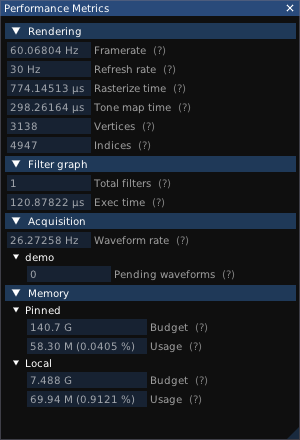
\includegraphics[width=7cm]{ng-images/dialog-perfmetrics.png}
\caption{Performance Metrics dialog}
\label{fig:perfmetrics}
\end{figure}

\subsection{Rendering}

Displays render loop framerate, monitor refresh rate, total time spent last frame in the rasterization and tone
mapping shaders, and the number of vertices and indices drawn as Vulkan geometry. Note that waveforms are drawn by a
compute shader and do not contribute towads the vertex/index totals, other than a single textured rectangle used for
displaying the shader output.

\subsection{Filter graph}
Number of filter blocks in the current graph, and run time for the most recent evaluation of the
filter graph.

\subsection{Acquisition}

Displays the acquisition rate, in waveforms per second. This data is collected using a rather simple mechanism and
may not be usefully accurate if multiple trigger groups are in use.

Additionally, this section displays the number of pending waveforms for each instrument (waveforms which have been
acquired but not yet passed to the filter graph). This number should normally be flickering between zero and one if
acquisition is active and zero otherwise; larger values indicate that the instrument is supplying data faster than
ngscopeclient can process it.

\subsection{Memory}

Displays the total amount of available pinned memory (CPU-side memory eligible to be shared with the GPU) and local
memory (memory attached to the GPU), as well as the amount of each currently in use.

%%%%%%%%%%%%%%%%%%%%%%%%%%%%%%%%%%%%%%%%%%%%%%%%%%%%%%%%%%%%%%%%%%%%%%%%%%%%%%%%%%%%%%%%%%%%%%%%%%%%%%%%%%%%%%%%%%%%%%%%

\section{Preferences}
\label{dlg:preferences}

The Preferences dialog allows you to configure various application settings which are not specific to a particular
experimental setup. It can be found under the \menustyle{Setup | Preferences} menu.

\begin{figure}[H]
\centering
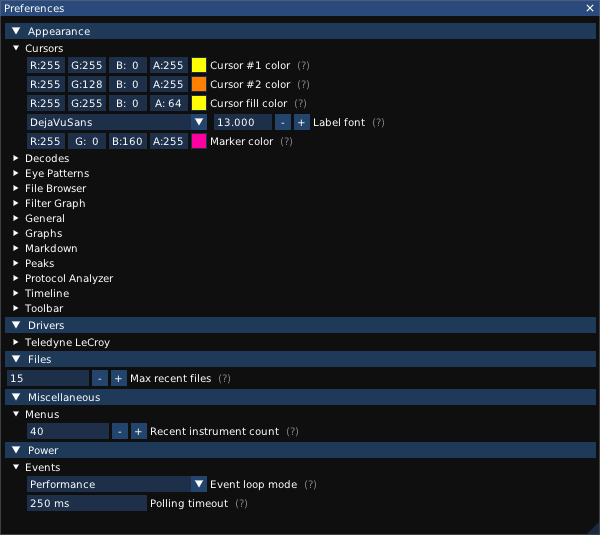
\includegraphics[width=7cm]{ng-images/dialog-preferences.png}
\caption{Preferences dialog}
\label{prefs}
\end{figure}

\subsection{Appearance}

This section allows you to configure fonts, colors, and other display settings for the application.

% TODO: document all of these preferences once the list has stabilized a bit

\subsection{Drivers}

This section allows you to configure default configurations for various instrument drivers.

\subsubsection{Teledyne LeCroy}

\begin{itemize}
\item \emph{Force 16 bit mode} (default on): Always use 16-bit format for downloading data from the instrument, even if
it only has an 8-bit ADC. This doubles the amount of network bandwidth required and may reduce waveforms-per-second
performance, but provides smoother waveforms since the instrument performs DSP flatness correction leading to >256
possible output values in a given waveform.
\end{itemize}

\subsection{Files}

\begin{itemize}
\item \emph{Max recent files}: Specify the number of files to display under the \menustyle{File | Recent Files} menu.
\end{itemize}

\subsection{Miscellaneous}

\subsubsection{Menus}

\begin{itemize}
\item \emph{Recent instrument count}: Specify the number of recently used instruments to remember
\end{itemize}

\subsection{Power}

\subsubsection{Events}

This section provides settings allowing power vs performance tradeoffs. The default settings are appropriate for a
desktop or laptop running on AC power; if running on a laptop with battery power you may wish to tune these to extend
battery lifespan.

\begin{itemize}
\item \emph{Event loop mode}: Controls the operating mode for the main application event loop.
\begin{itemize}
\item In Performance mode, run at the screen refresh rate. This allows for the highest possible waveform processing rate
and the smoothest interactivity, but may waste energy if you are spending a lot of time looking at the screen without
actively acquiring or processing waveforms.
\item In Power mode, run at a greatly reduced frequency (default 4 Hz but configurable by the Polling Timeout setting)
unless a redraw is triggered by mouse movement or keyboard input. This will limit the rate of waveform acquisition and
lead to a slightly jerkier user interface, but saves power.
\end{itemize}
\item \emph{Polling timeout}: If the event loop is in Power mode, specifies the timeout before the event loop will run
if there is no user input.
\end{itemize}

%%%%%%%%%%%%%%%%%%%%%%%%%%%%%%%%%%%%%%%%%%%%%%%%%%%%%%%%%%%%%%%%%%%%%%%%%%%%%%%%%%%%%%%%%%%%%%%%%%%%%%%%%%%%%%%%%%%%%%%%

\section{Speed Bump}
\label{dlg:speedbump}

The Speed Bump dialog is displayed when loading a session file, prior to committing changes to the instrument, if:

\begin{itemize}
\item The session file contains any user-created notes on the lab setup
\item Any of the instrument settings in the session file do not match the current configuration of the corresponding
instrument, and the direction of the change has potential to cause damage to the instrument or DUT (increasing output
voltage, removing input attenuation, etc).
\end{itemize}

This is intended as a safeguard to prevent damaging hardware by accidentally loading the wrong session file. It also
provides an opportunity to confirm that you have re-created the original experimental setup exactly if you are
switching a lab bench between multiple projects and using saved sessions to restore instrument state.

Pressing the Abort button cancels loading of the session without applying any of the potentially dangerous changes.
The instruments may be partially reconfigured in this state, as some changes (such as sample rate or memory depth
configuration) are always safe to make and thus may execute prior to the warning being displayed.

Pressing the Proceed button allows ngscopeclient to proceed with loading the session and reconfiguring hardware. You
must check the ``I have reviewed the instrument configuration" box in order to enable the Proceed button.

\begin{figure}[H]
\centering
\bigimage{ng-images/dialog-speedbump.png}
\caption{Speed Bump dialog}
\label{speedbump}
\end{figure}

%%%%%%%%%%%%%%%%%%%%%%%%%%%%%%%%%%%%%%%%%%%%%%%%%%%%%%%%%%%%%%%%%%%%%%%%%%%%%%%%%%%%%%%%%%%%%%%%%%%%%%%%%%%%%%%%%%%%%%%%

\section{Timebase}
\label{dlg:timebase}

The Timebase dialog allows you to configure sample rate and record length for oscilloscopes. It also provides control
over functionally similar ``what to look at" settings for other instruments, such as center frequency and span for
spectrum analyzers or sweep range and point count for vector network analyzers.

It can be found under the \menustyle{Setup | Timebase} menu.

\begin{figure}[H]
\centering
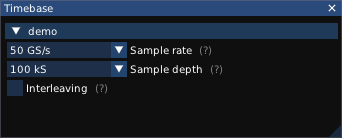
\includegraphics[width=7cm]{ng-images/dialog-timebase.png}
\caption{Timebase dialog}
\label{timebase}
\end{figure}
